\section{Tsetlin Machine Model Training and Serialization}
\label{sec:model_rep}

\subsection{Training Configuration and Host-Side Execution}
\label{sec:training_config}

The TM model is trained on a host PC using the fast-tsetlin-machine repository \cite{cair_fast_tm_mnist}, a C implementation of the TM that uses bitwise operators for increased training and inference speed. The repository provides a binarized form of the MNIST dataset, with a threshold value of 0.3, meaning all pixel values above 0.3 are set to 1, and the remaining pixels are set to 0. The hyperparameters used during training are shown in Table \ref{tab:tm_hyperparams}.

\begin{table}[H]
\centering
\caption{Training hyperparameters for the MNIST TM model.}
\label{tab:tm_hyperparams}
\begin{tabular}{ll}
\hline
Parameter & Value \\ \hline
Clauses per class & 2000 \\
Threshold $T$ & 50 \\
Sensitivity $s$ & 10.0 \\
TA states & 8 \\
Epochs & 1 \\
Classes & 10 \\ \hline
\end{tabular}
\end{table}

As accuracy is not a priority in this project, only a single training epoch used to save time. The focus is instead on inference performance, meaning the only concern is that the different inference programs evaluated later are running the same model and achieve the same accuracy.

The TM training algorithm relies on stochastic feedback, which is implemented using floating-point arithmetic in the fast-tsetlin-machine repository. The NEORV32 does not include a floating-point unit, meaning all floating-point computations are very slow \cite{Nolting2024Datasheet}. Due to this it was decided that while entirely possible to implement, on-chip training would be outsite of the scope of this work as the possible performance gains introduced by custom instructions would be negligible compared to the overall training time.


\subsection{Action Bit Plane Extraction}
\label{sec:action_bit_plane}

During training of the TM, the full model is stored, including TA states, meaning 8 bits per literal. As mentioned in Section \ref{sec:tm_ta}, only the action bit (include or exclude) of each literal, or the action bit plane, is needed to perform inference. While discarding the state bits hinders on-chip learning, this reduces model size by a factor of the number of TA states, or in this case 8. 

Custom functions were added to the training repository to extract the action bit plane and serialize it to a binary a binary file \textcolor{red}{cite appendix}. For each class and each clause, the function writes 25 positive literal words followed by 25 negative literal words, each word being a 32-bit unsigned integer.

\subsection{Literal Layout and the Mixed-Word Problem}
\label{sec:literal_layout}

The internal \texttt{ta\_state} array in the fast-tsetlin-machine repository stores the action bit plane as a packed bitfield across \texttt{LA\_CHUNKS} 32-bit words per clause, with $\texttt{LA\_CHUNKS} = (\text{\#literals}\div 32)$ \cite{cair_fast_tm_mnist}. For MNIST with 784 features, the literal vector contains 1568 bits (784 positive and 784 negative literals), requiring 49 32-bit words to store all literal actions. Since $784 = 24 \times 32 + 16$, the positive and negative literal regions do not fall on a 32-bit word boundary. Word 25 contains the 16 remaining positive literal bits in its  lower half and the first 16 negative literal bits in its upper half. This mixed word makes it impossible to directly separate positive and negative literal masks on a per-word basis, which is required by the CFU instruction designs described in Section~\ref{sec:cfu_impl}.


To resolve this, a zero-padded layout was used when serializing the model. Each clause is stored as 25 positive literal words followed by 25 negative literal words, for a total of 50 words per clause. The boundary words (25 and 50) are split in half, with the lower 16 bits containing literals and the uper 16 bits zeroed. This is illustrated in Figure \ref{fig:mixed_word}.

\begin{figure}[H]
    \centering
    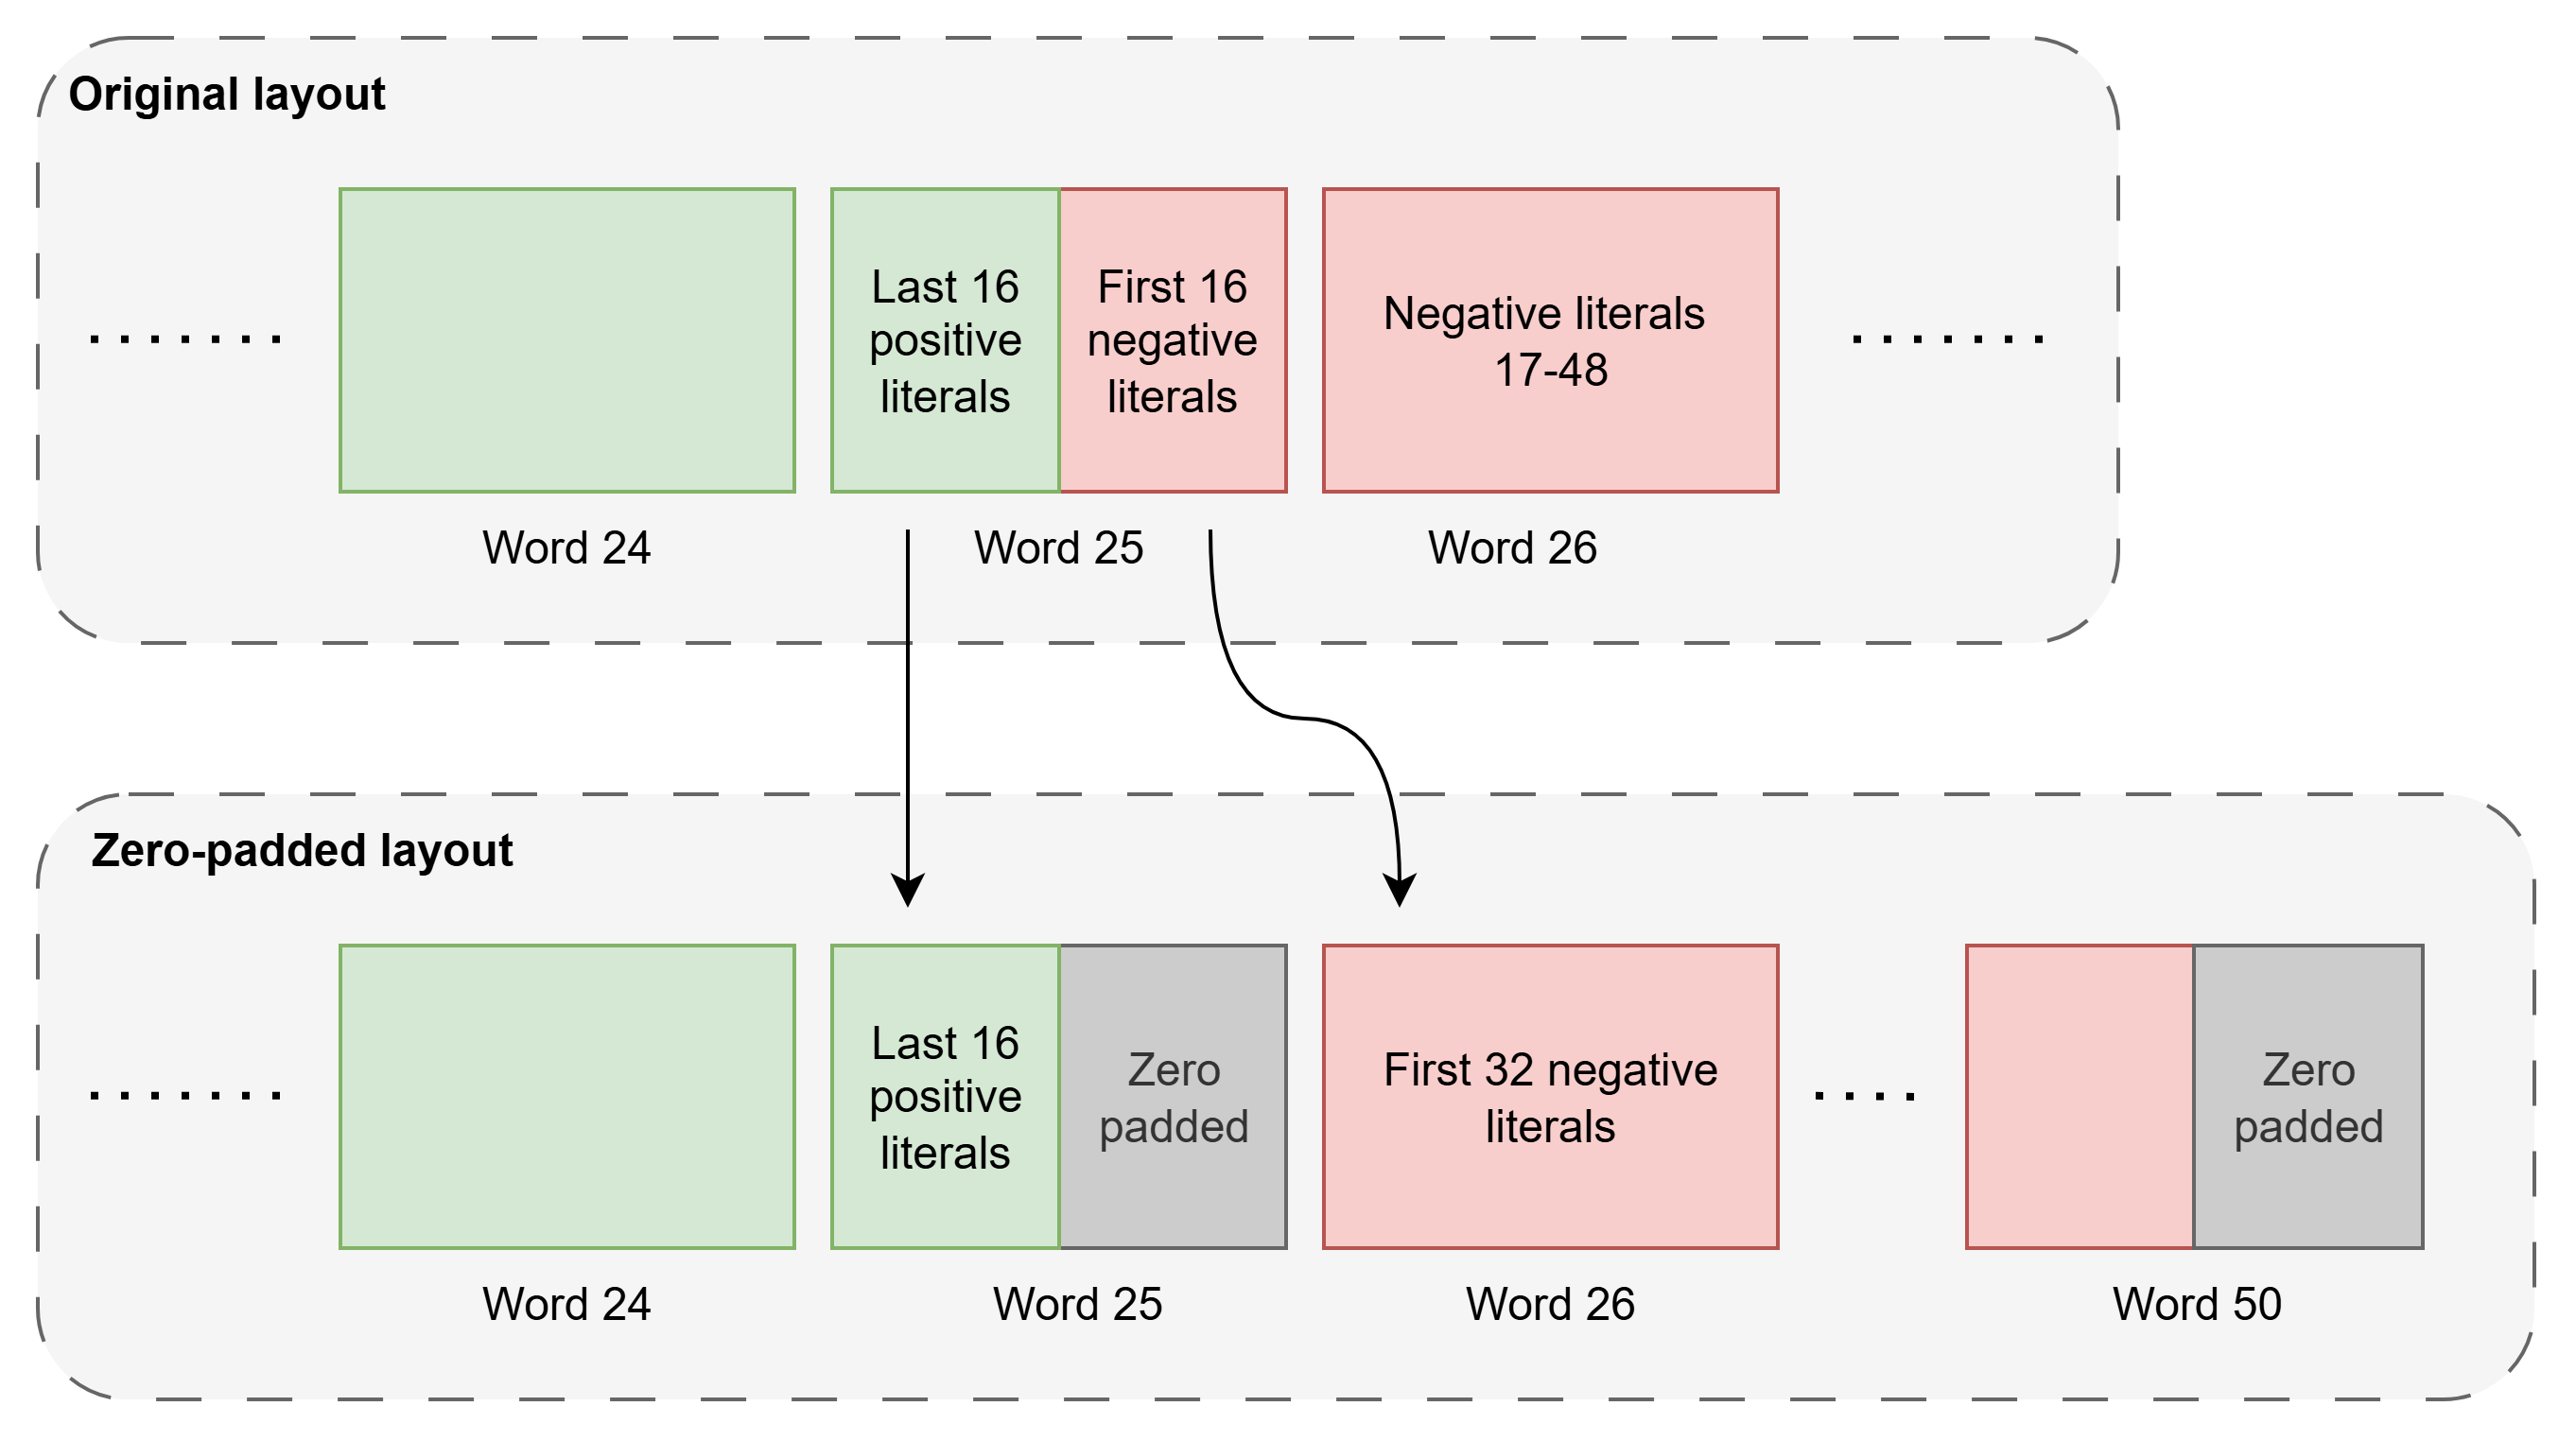
\includegraphics[width =1.0\textwidth]{Figures/mixed_word_problem.png}
    \caption{Comparison of the original 49-word literal layout and the 
    zero-padded 50-word layout. The zero-padded layout splits word 25 so that all words contain either only positive or only negative literals.}
    \label{fig:mixed_word}
\end{figure}

The resulting model sizes for the two layouts are summarized in
Table~\ref{tab:model_sizes}.

\begin{table}[H]
\centering
\caption{Model sizes for the original and zero-padded literal layouts.}
\label{tab:model_sizes}
\begin{tabular}{c|ccc}
Layout      & Words per clause & Total size (bytes) & Total size (MB) \\ \hline
Original    & 49               & 3 920 000 bytes    & $\approx3.74\text{ MB}$          \\
Zero-padded & 50               & 4 000 000 bytes    & $\approx3.81\text{ MB}$     
\end{tabular}
\end{table}

Both layouts exceed the capacity of the processor's internal memories by a large margin, necessitating the multi-tier storage architecture described in Section~\ref{sec:hw_config}.